\documentclass[12pt, a4paper]{article}

\usepackage[utf8]{inputenc}
\usepackage[T1]{fontenc}
\usepackage{fullpage}
\usepackage{hyperref}
\usepackage[parfill]{parskip}
\usepackage{natbib}
\usepackage{url}
\usepackage{amsmath}
\usepackage{graphicx}
\graphicspath{{images/}}
\usepackage{vmargin}

\title{The Delivery Man Lab Assignment}	% Title
\author{André Le Blanc, Joel Wallin}
\date{\today}			

\makeatletter
\let\thetitle\@title
\let\theauthor\@author
\let\thedate\@date
\makeatother

%----------------------------------
% Wizard stuff
%----------------------------------
\begin{document}

\begin{titlepage}
	\centering
    \vspace*{0.5 cm}
    %\includegraphics[width=5cm,height=5cm,keepaspectratio]{deadrop_text.png}\\[0.5 cm]
    %\includegraphics[width=5cm,height=5cm,keepaspectratio]{deadrop_logo.png}\\[1 cm]
    \textsc{\huge Artificial Intelligence (1DL340) fall 2016}\\[2.0 cm]
	\textsc{\Large Version 1, \today}\\[0.5 cm]
	\rule{\linewidth}{0.2 mm} \\[0.4 cm]
	{ \huge \bfseries \thetitle}\\
   
	\rule{\linewidth}{0.2 mm} \\[1.5 cm]
    
    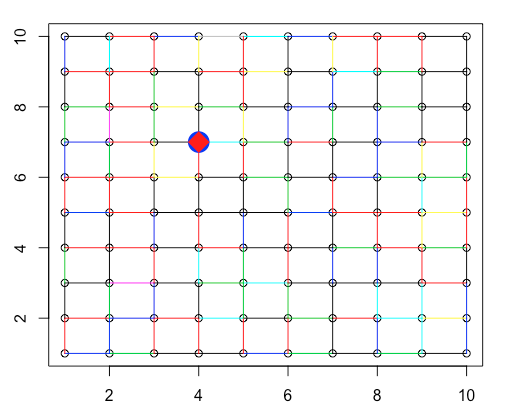
\includegraphics[width=10cm,height=5cm,keepaspectratio]{ADONE.png}\\[0.5 cm]
    
    \textsc{\Large Lab Group 14:}\\[0.5 cm]
	\begin{minipage}{0.4\textwidth}  
    \begin{align*}
	&\text{André Le Blanc}    &&\text{910930-3850}\\
	&\text{Joel Wallin}  &&\text{941123-3134}\\
	\end{align*}
	\end{minipage}\\[2 cm]
\end{titlepage}


\newpage
\tableofcontents
\newpage

\section{Introduction}

For this lab assignment we wrote a program that guides a deliveryman through a grid to his packages and then guides him to the package's destination. During the simulation traffic conditions change each step of the simulation. This means that the program has to recalculate the optimal route of the deliveryman for each step of the simulation using the A* algorithm. This means that the program will always find the optimal route between its location and its destination.

The user can watch the grid and the deliveryman traversing the grid with the help of a graphical user interface. Once the simulation is over the program prints the value of the number of steps it took for the deliveryman to complete his tasks. 

By running multiple simulations with different variations on the A* algorithm and different algorithms for choosing which package to pick up next we have collected data on the efficiency of these algorithms.

\section{Tools and methods}

The programming language used for this assignment was R. R is a high level multiparadigm language designed for statistical computing. After a short attempt using Emacs and UNIX shell we settled for R studio as our development environment. 

We used GIT for version control and sharing files within the group. 

\section{Algorithms}

\subsection{A*}

\subsubsection{A theoretical overview of A*}

A* is a pathfinding algorithm developed from Dijkstra’s algorthim in 1968 by Nils Nilsson, Bertram Raphael and Peter Hart. It promises to find the shortest path between two nodes in a well defined system if such a path exists. 

A* is a best first search algorithm meaning that it explores a graph or a weighted graph by expanding the most promising node. At every iteration of A* the program determines which partial path is most promising and expands that path. 

At the heart of the A* algorithm we have the following function :

\begin{center}
$f(n) = g(n) + h(n)$
\end{center}

In this function n represents the last node on a path. g(n) is the cost of getting to that node from the starting node. h(n) is a heuristic for the distance between node n and the destination. 

A* tries to minimize the f(n) function and chooses to expand on the nodes where the function f(n) has the lowest value. 

g(n) is generally obtained by adding together the costs of getting to each node on the shortest path between the starting point and node n. 

finding a good implementation of h(n) is a science in itself. If the heuristic between node n and the destination always is zero then:

\begin{center}
$f(n) = g(n)$
\end{center}

This means that A* will be an implementation of Dijkstra’s algorithm since A* is Dijkstra’s algorithm with a heuristic that helps A* chose the most efficient node to expand. A* will still find the shortest path but the algorithm will be more costly to run.

If h(n) has a higher value but the value is still lower than the cost of going from node n to the destination the algorithm will be more efficient expanding fewer nodes that are unnecessary to expand. 

In an ideal situation h(n) is equal to the cost of traveling from node n to the destination. In this case A* will only expand nodes that are on the path between n and the destination. 

In the unfortunate case where h(n) is greater than the cost of getting from node n to the destination it is possible that the A* algorithm finds a path that is less efficient than the optimal path between n and the destination. There for it is extremely important that:

\begin{center}
$h(n) \leq g(n)$
\end{center}

Finding an h(n) function that gives as large as possible value without ever exceeding g(n) can be one of the hardest parts of implementing A*.



\subsubsection{Our implementation of A*}

% Things to write about: 
% 1. Briefly about different heuristics and A* strategies used.
% 2. How we break ties.
% 3. Does it stand still (wait)?
% 4. Talk about what our algorithm does, ie. it finds the closest package and then delivers it. It does not step through all the possible combinations of paths it can take and the goes and delivers every package.

\subsection{Choosing which package to go to}

\section{Results}

In order to measure the effectiveness of different heuristics, A* strategies and not A* strategies, hundreds of different runs were executed with these varying parameters. Then the different strategies could be evaluated by looking at the expected value and standard deviation of their series of results (number of steps). 

Using Manhattan distance or Euclidean distance as the heuristic did not yield any noticeable improvements. Strategies that deemphasized the $g$ cost in the A* algorithm did perform worse and penalizing high $g$ costs led to the car zigzagging slightly more and avoiding costly paths, which narrowly improved its performance. Another benefit of some of these strategies were a slightly shorter execution time.

%insert graph of penalized g cost

Waiting at a node when the $g$ cost is high did not better the performance either. The car would stand still for too long, negating the benefits of waiting. Giving the car a chance $p$ (different values for $p$ were used, ranging from 5\% to 40\%) of waiting if the cost was high still made it perform worse than not waiting.

%insert waiting graph here

The final chosen setup was using the Manhattan distance as the heuristic and slightly penalizing high $g$ costs. 1,000 runs were executed and the results of those can be seen represented as a histogram and box graph below. The expected value of the algorithm is: 123.456 steps and the standard deviation was: 12.34. 

%insert the histogram and box graph

\section{Discussion}

The implemented A* algorithm yields a better result than a person stepping through the graph without extensive analysis of the grid's state. As the algorithm can both fast and accurately measure a decent path to its destination. The algorithm could have done much more extensive analysis, ex. comparing paths between different packages and choosing the order of packages which provides the shortest path. This was not implemented due to shortage of time.

In this problem, the $g$ cost grows fast as the algorithm traverses the grid, while the heuristic grows linearly. The $g$ costs therefore is emphasized more when calculating the $f$ value of a node. This makes the car follow low $g$ costs to a greater extent. But the path the car takes is still straight for the most part due to detours not being evaluated as being worth it. This can be explained due to the design of the problem. For every iteration of the program, the chance that the cost of a road will change is calculated through a uniform distribution of random numbers. Where the chance that the cost will increase is 10\% and decrease is 5\%. For every iteration, the road conditions will therefore on average worsen. This also explains why waiting is almost never beneficial.

\section{Conclusion}


\end{document}
